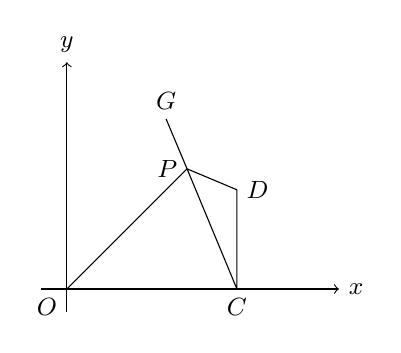
\begin{tikzpicture}[scale=.72, every node/.style={font=\small}]
  \coordinate (O) at (0,0); \coordinate (C) at (3,0);
  \coordinate (D) at (3,1.75); \coordinate (G) at (1.75,3);
  \coordinate (P) at (2.12,2.12);
  \draw[->] (-.45,0)--(4.8,0) node[right] {$x$};
  \draw[->] (0,-.4)--(0,4) node[above] {$y$};
  \draw (O)--(P) (P)--(C) (P)--(D) (P)--(G) (C)--(D);
  \foreach \p/\pos in {O/below left,C/below,D/right,G/above,P/left}
    \node[\pos] at (\p) {$\p$};
\end{tikzpicture}
